\Chapter{Ellenfelek viselkedésének modellezése}
\label{Chap:viselkedes}

A mesterséges intelligencia útvonalkeresés részéről már szó volt a korábbiakban, viszont nagyon fontos, hogy az ellenfeleknek egyéb tulajdonságokat adjunk, ezzel érdekesebbé téve a játékot. Szüksége van minden ellenfélnek egy célra, ami alapjában véve az, hogy megtámadják a játékost, viszont bizonyos szituációkban ez megváltozik, így kapunk még élethűbb viselkedést. Ez a fejezet ezen elemek bemutatásáról szól.

\section{Viselkedés bemenetei és kimenetei}

Ahhoz hogy az ellenfelek viselkedését modellezzük, különböző bemenetekre és kimenetekre van szükség.

\subsection{Bemenetek}
Bemenetként az ellenfél szemszögéből számít a játékostól való távolság, az aktuális életerő, a lőszer mennyisége, hogy a játékos benne van-e a látótérben, illetve hogy egyedül kell-e neki szembeszállni a játékossal, vagy többen vannak. Ezek a bemenetek egymástól is függhetnek. Ha a játékostól való távolság kisebb, mint egy előre definiált érték, és nem egyedül vannak, akkor közelítsenek és támadjanak, viszont ha egyedül van, akkor próbáljon menekülni. Figyelembe veheti azt is, hogy milyen hatékony fegyver van a kezében, az életereje vagy lőszere egy előre definiált érték alatt van-e, és ezek függvényében támad, keres életerőt vagy lőszert. Az ilyen típusú adatok definiálásának legjobb módja, ha az ellenféltípusokhoz hozzárendelünk különböző tulajdonságokat, így kialakíthatjuk, hogy melyik miben jó, és miben rossz. Ezt nevezzük karakterisztikának.

\begin{figure}[h]
\centering
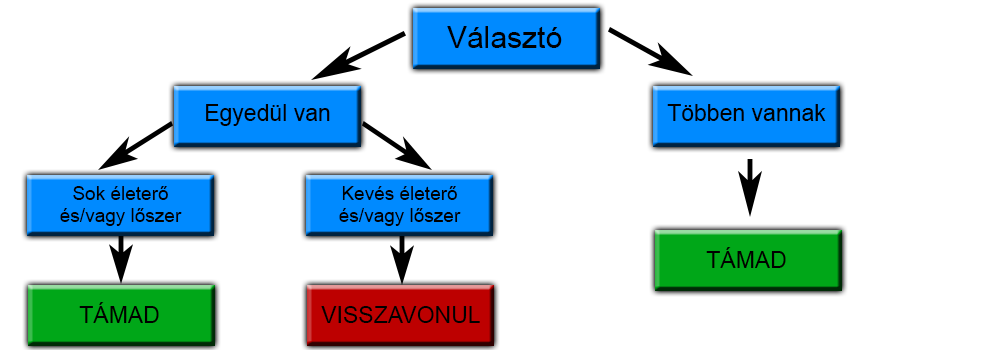
\includegraphics[scale=0.38]{kepek/viselkedes.png}
\caption{Az ellenfél egy lehetséges viselkedése}
\label{fig:behavior}
\end{figure}

\subsubsection{Adott ellenfél karakterisztikája}

\begin{tabular}{r|l}
Név & Az ellenfél neve. \\
Támadóképesség & Ellenfél képességei támadás közben.\\
&> 0.0 \& < 0.15 = Nem mozdul.\\
&>= 0.15 \& < 0.5 = Csak előre és hátra mozog.\\
&>= 0.5 \& < 1.0 = Körbe-körbe megy.\\
&> 0.6 \& < 1.0 = Véletlenszerű mozgás irányváltással.\\
&> 0.4 \& < 1.0 = Visszavonuláskor is fedezze magát lövéssel.\\
Agresszió & Az ellenfél agressziója.\\
Neme & Férfi, nő, vagy egyéb teremtmény\\
Célzóképesség & Fegyverenként különbözhet.\\
&> 0.0 \& < 0.9 = Az ellenfél mozgása hatással van a célzásra.\\
&> 0.4 \& <= 0.8 = Ellenfélmozgás követése.\\
&> 0.8 \& <= 1.0 = Várható felbukkanás helyének figyelése.\\
&> 0.6 \& <= 1.0 = Környezeti elemek felhasználása sebzésre.\\
Guggolás & Guggolás gyakorisága.\\
Ugrás & Ugrás gyakorisága.\\
Forgás & Forgás sebessége (reflex).\\
Reakcióidő & Miután meglát, mennyi idő telik el az első lövésig.\\
Lövéspontosság & 0 és 1 közötti érték, a lövés szórását adja meg.\\
Bosszú & Az ellenfél bosszúállósága.\\
\end{tabular}

\subsection{Kimenetek}

A bemeneti adatok alapján a program egy modulja kiértékeli az eseményeket, és annak kimeneti értékei határozzák meg a következményeket. Minden kimenet egy végrehajtható akciót jelöl (támadás, menekülés, életerő vagy lőszer töltés). A döntési fa az csak az állapotot határozza meg. Minden iterációban ki kell értékelni, és minden lehetséges esethez meg kell írni azt a kódrészt, ami az adott cselekvésfolyamatot elindítja. \Aref{fig:behavior}-es ábrán kékkel vannak jelölve a bemeneti paraméterek, zölddel és pirossal pedig azok következményei, vagyis a kimenetek.

\subsection{Program: Viselkedés}

Ezen a program elkészítésével az volt a célom, hogy minél egyszerűbben, vizuálisan lehessen bemutatni az ellenfelek viselkedését. A termelésinformatikában ennek az algoritmusnak a segítségével különböző döntési tényezőket lehet definiálni, hogy a robot azoknak megfelelően cselekedjen. Jelen esetben a játékost fehér, az ellenfeleket piros, a biztonságos pontokat kék négyzet jelöli. A biztonságos pontok azok a helyek, ahova egy ellenfél vissza tud vonulni, ha a játékos megmozdul. Minden ellenfél a korábban leírtaknak megfelelően rendelkezik egy karakterisztikával, amely minden esetben két tulajdonságból áll, a sebességből, és a félelemfaktorból. Utóbbi azt határozza meg, hogy ha megmozdul a játékos, mekkora legyen az a sugár, amelybe ha egy biztonságos pont beleesik, visszavonuljon. Ha több pont esik az adott sugárba, akkor azok közül is a legközelebbit választja.

A félelemfaktor függ az ellenfél sebességétől is, tehát gyors ellenfél esetén csak alacsony értékeket, lassú ellenfél esetén pedig csak magas értékeket vehet fel, ezzel életszerűbbé teszi a viselkedést. A mintaprogram felépítése \aref{fig:behavior_uml} ábrán látható.

\begin{figure}[h]
\centering
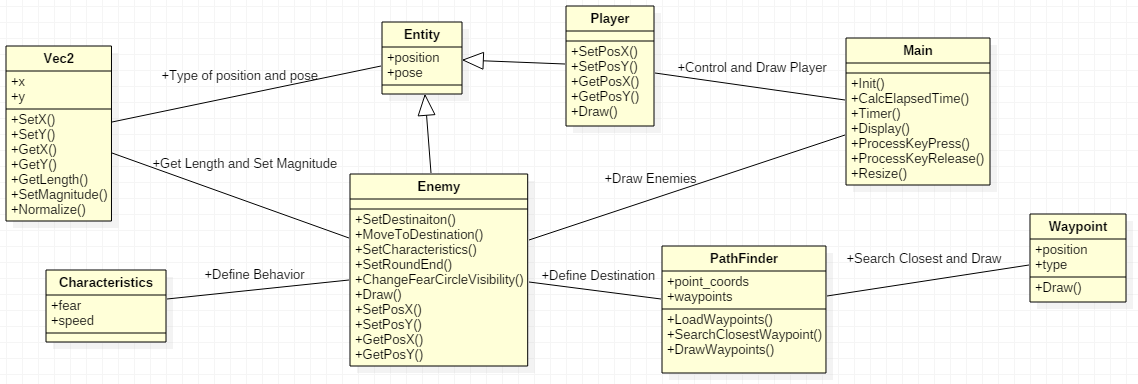
\includegraphics[scale=0.5]{kepek/behavior_uml.png}
\caption{A viselkedést bemutató program felépítése}
\label{fig:behavior_uml}
\end{figure}

\Aref{fig:behavior_settings} ábrán látható módon, az elindítás után minden ellenfélnek véletlenszerűen generál egy karakterisztikát, olyan módon, hogy a sebességet és a félelemfaktort beállítja egy adott értékre. A felhasználónak lehetősége van ezeket újragenerálni, illetve minden ellenfélnek a félelemfaktorát vizuálisan megjeleníteni, amely \aref{fig:behavior_demo} ábrán látható.

\begin{figure}[h]
\centering
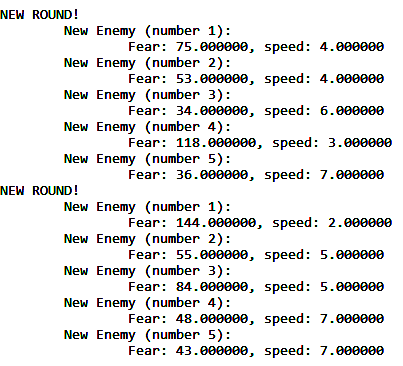
\includegraphics[scale=0.8]{kepek/anim_random_values.png}
\caption{Az ellenfelek félelemfaktora}
\label{fig:behavior_settings}
\end{figure}

\begin{figure}[h]
\centering
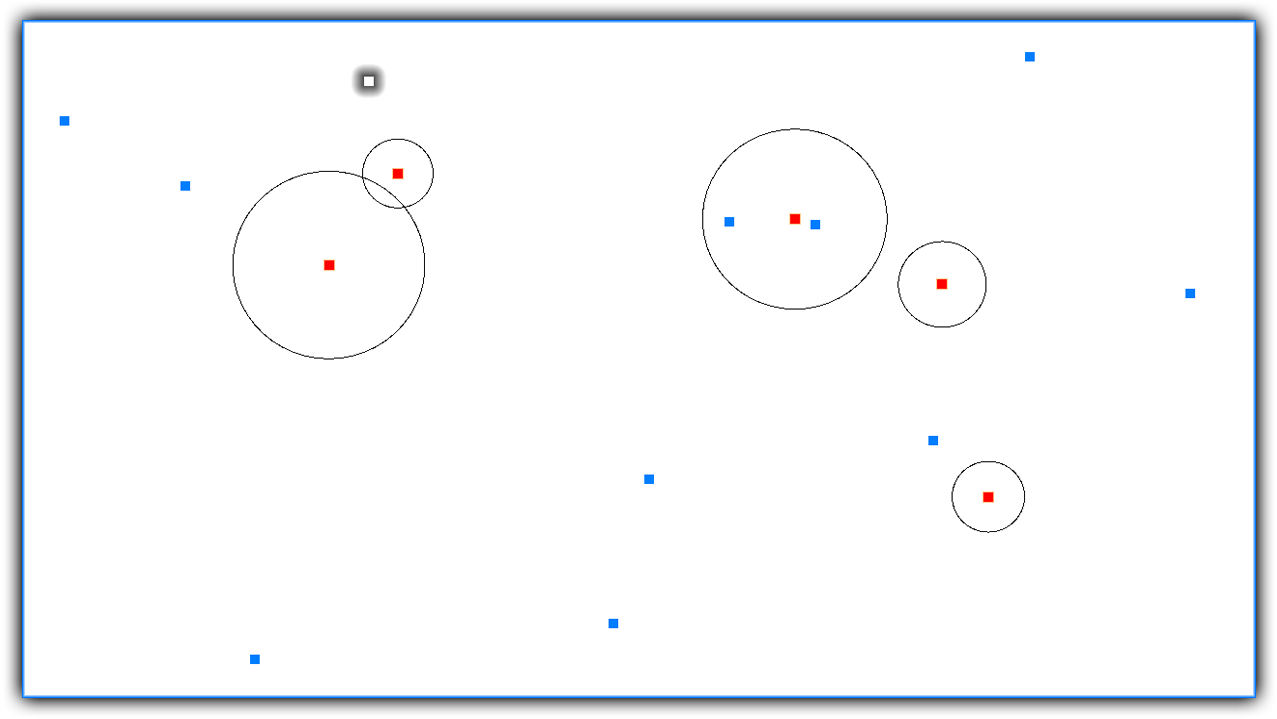
\includegraphics[scale=0.42]{kepek/behavior_demo.png}
\caption{Az ellenfelek félelemfaktora}
\label{fig:behavior_demo}
\end{figure}

\section{Véletlenszerű tényezők}

A játékban el vannak helyezve különböző használható elemek, amelyek kihatással vannak a játékmenetre. Viszont az, hogy annak milyen mértékben van hatása pozitív irányban, csak akkor derül ki, ha már felvettük azt. Különböző típusú elemek léteznek, amiket a mesterséges intelligencia által vezérelt ellenfelek is tudnak hasznosítani. A játéktéren találhatunk életerőre, lőszerre és csapda megjelenési idejére hatással levő elemeket.

\subsection{Konkrét megvalósítás}

Az életerő és a lőszer megvalósítás szempontjából egy egész (integer) típusú, a csapda megjelenési ideje pedig egy tört (float) szám. A felvehető elemek ezeket az értékeket módosítják különböző mértékben. Ezek egyikének megvalósítása \aref{fig:health} ábrán látható.

\begin{itemize}
\item Életerőt véletlenszerűen 10, 25 vagy 50\%-kal növelheti. 
\item Lőszerhez véletlenszerűen adhat 15, 30, vagy 50 darabot.
\item Csapda megjelenési idejét véletlenszerűen növelheti 25, 50 vagy 100\%-kal.
\end{itemize}

\begin{figure}[h]
\centering
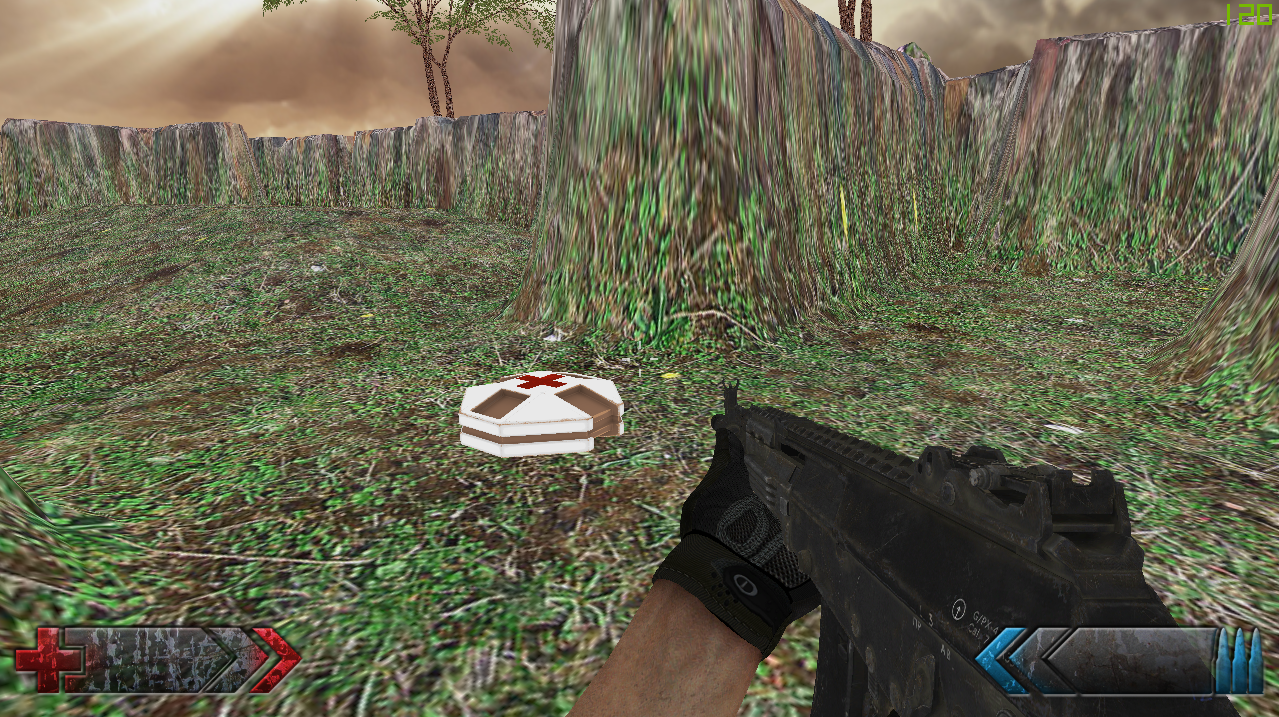
\includegraphics[scale=0.4]{kepek/health.png}
\caption{Egy felvehető elem a játékban}
\label{fig:health}
\end{figure}

